\section{Detection Mechanism}
\label{sec:detection}

%  \mn[Stef]{Somehow the word manipulation seems wrong here, both approaches are dropping, one just also drops the chunk information, the other one only the chunks as such; manipulation makes it sound as if nodes produce false BMs}
In this section, we explain our proposed two-fold detection mechanism, starting with an overview of the different steps followed by a detailed description of each step.  
The goal of the detection algorithm is to restore the user's satisfaction by replacing and identifying malicious peers that refuses to forward chunks as dictated in the protocol.

On a high level, we utilize an approach for malicious nodes that do not update their buffer-maps, an attack behavior we denote by \drop. 
We show through the rest of the section the concept behind how peers can identify potential sources for their lack of satisfaction in collaboration with other peers.     
% attack behavior we denote by \block, and a global (requires cooperation from peers) approach against malicious nodes that do not update their buffer-maps, an attack behavior we denote by \drop.
% Accordingly, when considering the detailed description of each step, the detection mechanisms naturally differs. 




\begin{table}[ht]
\center
\caption{Acronyms}
\begin{tabular}{|c|l||c|l|}
\hline

\bf{Var.} & \bf{Description}  & \bf{Var.} & \bf{Description} \\\hline\hline
$H_n$ & headnodes in a complaint & $P_n$ & potential candidates list \\\hline
$x$ & no. of malicious peers & $\eta$ & mal. headnodes fraction\\\hline
$BM$ & buffer-map & $MN$ & (1-$\eta$) non-headnodes mal. peers\\\hline
$\sat$ & peer satisfaction level & $\satThres$ & satisfaction threshold \\\hline
$\minP$ & min. drop responses & $\minDR$ & \drop det. allowed\\\hline
\end{tabular}
\label{tab:acronyms}
\end{table}
%  \mn[Stef]{Table: I cleared up some inconsistencies in the table, we used multiple lower-case letters for satisfaction, but one upper-case letter for familiarity and guilt, it's macros, feel free to change back; added $\minP$. re-ordered to have similar variables in the same line; I don't get what $MN$ is}

\subsection{Mechanism Overview}
We present the underlying ideas of the detection mechanism in Figure~\ref{detection-blocks}.

When a malicious peer $m$ performs a \drop attack, benign peers $b$ are unable to immediately identify malicious behavior.
Specifically, $m$ never sends the actual $BM$ that represents the chunks it currently possesses, i.e., $m$ is only requesting chunks it already has.
Thus, detecting a violation in this case is not feasible. 
To that end, through the rest of the section, we describe how the detection mechanism handles \drop attack strategy based on this fact.

The detection consists of four steps, starting with an initial trigger of dissatisfaction at one peer and potentially terminating in the replacement of one or several headnodes. 
First, when a detection condition is triggered by peer $b$, $b$ sends a detection request to all peers in its neighbor list.
Second, each peer receiving a detection request prepares a reply according to the request type.
Third, the initiator $b$ decides based on the received responses if it should file a complaint with the source.
If $b$ decides to file the complaint, $b$ sends it on behalf of the participating peers in the detection request. 
Afterwards, the source verifies the complaint, reacts accordingly, and replies to $b$ detailing the steps taken. 

The reaction of the source is either the replacement of one or several headnodes and proposing other potential headnodes or the rejection of the removal request.
Finally, $b$ reacts based on the received reply from the source and then forwards the source's reply to the other participants in the complaint, who in turn do the same procedure.
The node $b$ bases its decision on whether to initiate a request or forward a complaint on a number of threshold parameters. 

Table~\ref{tab:acronyms} provides a list of the most important parameters governing the attack strategies and the detection mechanisms. 


% \subsection{Drop vs.\ Manp Detection}
% \mn[Stef]{I think I added the equivalent content at the end of the section intro, decide where you want to cut it}
% Before detailing the four steps of the detection mechanism, we point out the critical differences between \drop and \block.
% 
% 
% 
% In contract, in a manipulation or outdated chunks scenario, $m$ is eventually suspected as $b$ already expects the requested chunk from $s$.
% Note that a peer might be overloaded due to a tight upload bandwidth or serving a lot of peers and thus, not able to serve all the requests.
% Accordingly, the detection mechanism should differentiate between a malicious manipulating peer and an overloaded peer, which is discussed in Section~\ref{Detection-Trigger}.
% To that end, through the rest of the section, we describe how the detection mechanism handles both cases: \drop and \block detection.

\begin{figure}
 \centering
 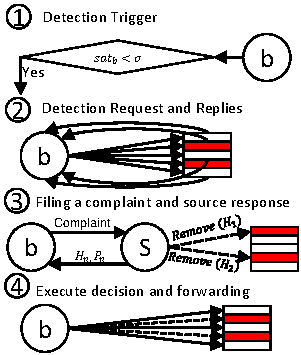
\includegraphics[width=5.5cm,height=6cm]{./Figures/detection.pdf}
  \caption{Detection process for \drop. $S$ represents the source peer.}
\label{detection-blocks} 
\end{figure}

\subsection{Detection Trigger}
\label{Detection-Trigger}
 Now we discuss how a peer decides on sending a detection request.
% In both behaviors, once $b$ decides on sending a detection request, it only sends to peers in its own neighbor list to check if those neighbors agree with it or not, disregarding the source if $b$ is a headnode.
% 
% Afterwards, as detailed in Section~\ref{Filing_a_Complain}, once $b$ receives its neighbors replies to the detection request, $b$ decides whether or not to fire a complaint to the source.

% \subsubsection*{Drop trigger}
As there is no identifying evidence of manipulation from any neighbor to $b$, the only factor that $b$ is concerned about is the satisfaction threshold $\satThres$.
The satisfaction of a peer is defined as the fraction of missed chunks, i.e., the continuity of the stream according to the $Hit/Hit+miss$ chunk ratio.
In details, $b$ decides to trigger a detection request only if:
\begin{enumerate}
 \item $b$'s current satisfaction level is less than the predefined threshold such that $\sat_b < \satThres$.
 \item Number of drop detections sent by $b$ in the last $t_{det}$ is $< \kappa$, where after $t_{det}$ peers are allowed to initiate $\kappa$ requests again.
 \item $b$ is not currently participating in another \drop detection process.
\end{enumerate}
The latter condition guarantees that any peer can not trigger or participate in multiple detection requests in parallel as: (a) frequently sending complaints will eventually overload the source,
and (b) the source is most likely processing another peer's dropping request that is most likely to enhance $b$'s satisfaction level as we discuss in Section~\ref{complaint_source}.
% Note that the detection request sent to $b$'s neighbors does not contain a certain suspect, hence, peers receiving a an empty suspect field request are aware that indeed it is a \drop request.
% \mn[Stef]{we never introduced the nature of the complaint, in particular not `suspect field'}

% \subsubsection*{Manp trigger}
% Whenever $b$ detects a manipulation event from $m$, $b$ stores the incident in its \textit{suspicious list}.
% $b$ decides to send a detection request if it was manipulated $\alpha$ times by $m$, i.e., the event counts for $m$ in $b$'s list equals $\alpha$.
% \mn[Stef]{can you be more exact about when exactly $b$ assumes there is manipulation happening? is it after not receiving a requested chunk after $k$ seconds?}
% Clearly, $b$ attaches the suspect ID in the detection request to its neighbors.
% 
% This condition essentially guarantees that any peer is not suspected instantly if it did not deliver the requested chunk, i.e., a benign peer might not deliver a chunk to the requester if it is already loaded due to serving other peers.
% Thus, when a benign peer is incapable of serving a request of another peer, it is already aware that the event was recorded and eventually, the serving peer will be under suspicious if it did not serve the upcoming requests from the same peer.
% In turn, the serving peer can assign higher priorities to serve requests for certain peers that have already manipulation logs about it.
% 
% In order to decrease the likelihood of malicious peers abusing the manipulation detection mechanism, participating peers in a \block request are requested to provide evidence of having the suspected peer in their neighbor list.
% To obtain such evidence, whenever peer $p_1$ is adding $p_2$ to its neighboring list, $p_2$ is requested to sign its entry in $p_1$'s neighbor list.
% Moreover, peers periodically request a fresh signatures from all other peers in their neighbor list.
% Accordingly, only peers with such fresh signatures from $m$ are allowed to participate in the complaint, i.e, as in fact, outdated signatures might indicates connections already removed from $m$'s neighboring list.
% This evidence is later needed for the source to decide about $m$, as detailed in Section~\ref{Filing_a_Complain}.
% \mn[Stef]{I would consider stating this somewhere else, maybe as step 0 of the detection or in the system model, as it is a prerequisite that happens before the any detection mechanism, having it here mixes up the temporal order}

\subsection{Replying to Detection Request \& Filing a Complaint}
\label{Filing_a_Complain}
Here we describe how a peer $d \in D$, where $D$ is the set of peers ($b$'s neighbors) who received a detection request from $b$, prepares a detection reply.
Afterwards, we discuss the procedure executed by $b$ to process the replies and accordingly, decides whether to file a complaint to the source or not.
Finally, we present how malicious peers aim at abusing the detection mechanism.
%  \mn[Stef]{mention again that $D$ contains neighbors of $b$, nobody will remember that from the overview}


\subsubsection*{Processing a detection request}
Once $d_b$ receives a detection request, it replies only with its current satisfaction level $\sat$.
Next, we describe how $b$ processes the values provided in the detection replies in order to reach a decision about firing a complaint to the source.

\subsubsection*{Filing a complaint}

$b$ will start processing the replies once all nodes in $D$ have replied or a time-out $t_{replies}$ since sending the request occurs. 
We assume that the source's address is publicly known and $b$ can send a complaint to the source directly.
% \subsubsection*{Drop request}
$b$ sends a complaint if the average satisfaction level indicated in the responses is below a threshold $\satThres$.
More specifically, if $\sat_1, \ldots , \sat_b, \ldots ,\sat_z$ is the satisfaction levels expressed in the $z$, after including $b$'s response, received responses,
$b$ files a complaint to the source if:
%  \mn[Stef]{do we consider $b$'s own satisfaction or only the nodes in $D$?}
\begin{align}
\label{eq:drop_satis_equation}
\frac{1}{z}\sum_{i=1}^{z} \sat_i< \satThres. 
\end{align} 
otherwise, $b$ either starts another detection request in case $\kappa >0$ in the interval of $\treply$, or waits till it is allowed to send another detection request.

Once $b$ decides on filing a complaint according to the aforementioned conditions, $b$ generates a complaint message to the source with the following information attached in the complaint message: 
(a) IDs of all participating peers, and (b) $\sat$ value in each reply.

\subsubsection*{Malicious abusing}

%  \mn[Stef]{I think we are mixing different content here, a description of the detection mechanism should first describe the detection complete mechanism, then you should talk about possible abuse}
As malicious peers collude with each other, they reply differently according to whether $b$ is benign or malicious.
We refer to a malicious detection initiator as $b_m$, $b_b$ otherwise.
Hence, we distinguish those two cases below. We refer to a malicious participant as $d_m$.

Intuitively, $d_m$ always aim at replacing more malicious nodes as headnodes while trying to keep already existing malicious headnodes.
Since malicious peers collude together, i.e., each malicious peer is aware about the current $\eta x$ ratio of malicious peers.
Hence, $d_m$ replies with $\sat=0$ in case the initiator is $b_m$. 
This is simply due to that malicious peers only initiate detection requests to increase the $\eta x$ ratio, thus, $d_m$ always aim at minimizing the aggregated $\sat=0$ to allow $b_m$ to file the complain.
Similarly, $d_m$ replies with $\sat=1$ if $b_b$ is the initiator in order to protect the malicious headnodes causing the dissatisfaction to $b_b$.


To that end, to prevent malicious peers from abusing the drop detection mechanism and cause an illusion at the source that a general dissatisfaction is detected, the following conditions are applied:
% \mn[Stef]{can we try to merge these with the constraints on $b$ starting the request, it is kindof repetitive like this}
\begin{enumerate}
\item At least $\minP$ have to participate in the request. 
 \item Each peer can at most generate or participate in maximum $\kappa$ drop complaints to the source per $\treply$.
%  \mn[Stef]{1000s seems arbitrary, introduce a parameter called for the length of the interval}
 \item No simultaneous generation or participation in more than one complaint is allowed to any peer, i.e., once $d$ is engaged in a detection process, it should wait till the final decision is reached.
\end{enumerate}
% \mn[Stef]{Who checks that these conditions hold? the source? $b$ should not be able to do so for the latter two, so why is that here}
Note that the source is responsible for checking that the last two constraints mentioned above hold.
If a peer violates one of them, the source attaches this peer's ID in the complaint reply so all other peers blacklist this peer.
 Although those conditions guarantee that malicious peers can not abuse the drop detection mechanism,
however, benign peers also have the same constraints, which might result in a benign peer not being able to eventually complain to the source.
For those reasons, as we further elaborate on Section~\ref{complaint_source}, once a drop detection complaint reaches the source,
the fraction of headnodes replaced can be large in order to maximize the likelihood of affecting a large fraction of the overlay, specially for peers who might not be able to complain to the source at the moment.


% In a \block request, $d_m$ replies with $\fami=1, \guilt=0, \sat=1$ in case the $s$ is a colluding malicious peer.
% Note that $d_m$ is incapable of providing fake $\fami$ values in its replies in case $s$ is benign due to the obligation of sending the signed proof that $s$ is indeed a neighbor of $d_m$. 

% 
% \subsection{Filing a Complaint}
% \label{Filing_a_Complain}
% %  \mn[Stef]{why `fire' and not file, which is the common word?}
% Next, we discuss $b$'s protocol for processing with the received detection replies.

%  \mn[Stef]{changed $i=0$ to $i=1$, check if that was intended}


% \subsubsection*{Manp request}
% In this simpler case where a certain suspect exists, $b$ decides to fire a complaint if the following conditions hold:
% 
% \begin{align}
% \label{eq:drop_familiarity_equation}
% \sum_{i=1}^{z} \fami_i > z/2
% \end{align}
% The condition in \ref{eq:drop_familiarity_equation} assures that at least more than half of the participant peers have information about the suspect, i.e., the suspect is an entry in their neighbor list.
% Next, for \textit{familiar} peers with the suspect, the aggregated \textit{Guilt} reported value must be greater than the maximum calculated value that can be reported by familiar peers, as stated in ~\ref{eq:drop_guilt_equation}.
% 
% \begin{align}
% \label{eq:drop_guilt_equation}
% \sum_{i=1}^{z} \guilt_i > \sum_{i=1}^{z} \fami_i*(\alpha-1)/2
% \end{align}
% Nevertheless, the same condition for \drop detection in \ref{eq:drop_guilt_equation} is also considered in a \block type.
% The reason for considering the satisfaction factor is to assure that the participating peers are currently unsatisfied, i.e., $d_b$ might have manipulation event for $m$ in their \textit{suspicious list} , however, $d_b$ is satisfied through other peers and no gain for it from firing a complaint and overload the source.

% \subsubsection*{Filing a complaint to the source}



\subsection{Processing a Complaint at the Source}
\label{complaint_source}
% At this point the source receives a complaint from $b$, the source decides on the next procedure depending on whether the complaint is a \drop or a \block.

At this point the source receives a complaint from $b$, the source decides on the next procedure depending on complaint request content.
The source conducts the following procedure:
\begin{enumerate}
 \item Divides the set of participating peers into two sets $H_n$ and $P_n$, where $H_n$ is assigned as the set of peers participating in the complaint that are already headnodes. 
%  \mn[Stef]{Isn't $H_n$ defined as complete list of headnodes in the table?}
 \item Removes all peers in $H_n$ from its neighbor set.
 \item Randomly connects to another $|H_n|$ peers. 
 The reason for not connecting to a fraction of the participating peers in the complaint is to avoid the probability that malicious peers are abusing the detection mechanism in order to get promoted to headnodes.
 \item Adds peers (excluding peers in $H_n$) from its neighbor list to $P_n$, where $P_n = NeighborList\setminus H_n$ ($NeighborList$ is the set of peers in a neighbor list). 
%  \mn[Stef]{confused on what $P_n$ is}
 \item Sends a \textit{Complaint Reply} to $b$ containing $H_n$ and $P_n$.
\end{enumerate}

% Note that the source can identify the request's type based on the suspect field, i.e., in case of no suspect attached, it is indeed a \drop complaint.

% \subsubsection*{Manp request}
% We start with the simpler case of receiving a \block request. 
% The source executes the following steps:
% \begin{enumerate}
%  \item Requests the neighboring list of $m$ to validate the familiarity of peers participating in the complaint, as discussed in Section~\ref{Detection-Trigger}.
%  \item If the above check is passed, the source removes the suspect $m$ from its neighbor list.
%  \item Saves the free entry in its list (after removing $m$) for $b$ to connect and be a headnode.
%  Accordingly, all the peers participating in the complaint will have a direct headnode ($b$) which remarkably enhances their satisfaction level.
%  \item $m$ is added to a blacklist, i.e., $m$ is not allowed to be a headnode again.
%  \item Generates a \textit{Complaint Reply} to $b$ confirming blacklisting $s$.
% \end{enumerate}

% \subsubsection*{Drop request}


\subsection{Processing a Complaint Reply \& Forwarding}

Finally, when $b$ receives the \textit{complaint Reply} from the source, $b$ performs the following procedure:
% which again differs based on the complaint type (\drop or \block).
% In a \block scenario, $b$ executes the following procedure:
% \begin{enumerate}
% %  \item Disconnects and blacklist the suspects.
%  \item Connects to the source, if, due to any other reason, the connection is not possible, $b$ connects to another random peer (excluding peers in $b$'s blacklist).
%  \item Forwards the \textit{Complaint Reply} to all peers who agree about $m$ being malicious, i.e., familiar peers with $G > 0$. \mn[Stef]{why not all neighbors?}
% \end{enumerate}
% Finally, the participating peers performs step 1 and 2 once they receive the forwarded reply.

% For a \drop scenario, $b$ follows the next procedure:
\begin{enumerate}
 \item Disconnects from all peers in $H_n$. Note that $b$ does not blacklist peers in $H_n$ from its neighbor list due to the fact that those peers are not proven malicious.
%  \mn[Stef]{what's the difference between disconnect and expel from a neighbor list?}
 \item Connects to $|H_n|$ peers from $P_n$, in case $|H_n|>|P_n|$, peers connect to $|P_n|+(|H_n|-|P_n|)random peers$.
\end{enumerate}
Similarly, $b$ forwards the complaint to the other participants, who in turn execute steps 1 and 2.

\subsection{General Notes}
The detection mechanism does not aim at expelling peers from the system.
The reason for the lack of harshness of the penalty associated with a detection lies in the potentially high false positive rate for headnodes that exhibit a low performance. 
These might be accidentally declared to be malicious peers due to not forwarding chunks sufficiently fast. 
% \mn[Stef]{In your original version, the explanation was specific to the drop case, I think this is a general problem but check if you want to revert to your version}

While removing such peers as headnodes is likely to benefit the system, it is not in our interest to ban them from the system. 
Indeed, the only peers that get blacklisted are those who violate the detection mechanism constraints, i.e., participating in more than a single request at a time or initiating more than $\kappa$.
% our mechanism neither entirely expels peers from the system nor even blacklisted them at the peers participating in the complaint neighbor list. 
% \mn[Stef]{don't really get the last few words, we did not define complaint neighbor list}

In general, the main target of the detection mechanism is to enhance the peers satisfaction level while minimizing: (a) peers replacements (through minimizing the number of detection requests initiated), (b) detection overhead, and (c) malicious peers chances to abuse the detection mechanism.
In the following section, we evaluate our mechanism's performance and accuracy, along with highlighting the attack's severity.
% \mn[Stef]{why is that only for the drop case?}

% Unlike in a \drop detection complaint, in a \block complaint, peers proved
% \mn[Stef]{again, they might just have a really low performance, why prove, you even state in the next sentence that it could be low resources}
% malicious throughout the detection process are eventually located at distant positions from the source (due to the removals occur once those peers are detected).\mn[Stef]{sounds grammatically wrong but I am not entirely sure what you want to say here}
% Hence, the reliance on those peers to deliver chunks to other peers is significantly minimized compared to headnodes peers or even headnodes neighbors (which positively impacts the overlay's satisfaction in case those peers are indeed malicious or due to low bandwidth, CPU resources or even an unreliable network connection).




